\documentclass[11pt,a4paper]{article}
\usepackage[utf8]{inputenc}
\usepackage[T1]{fontenc}
\usepackage{lmodern}
\usepackage{amsmath,amssymb,amsthm}
\usepackage{graphicx}
\usepackage{geometry}
\usepackage{hyperref}
\usepackage{siunitx}
\geometry{margin=1in}
\hypersetup{colorlinks=true, linkcolor=blue, citecolor=blue, urlcolor=blue}

\title{Optimization Methods for a Reduced PDE-Constrained Optimal Control Problem (Ex3)}
\author{Fachseminar Report}
\date{\today}

\begin{document}
\maketitle

\section*{Overview}
This report summarizes the mathematical formulation, discretization, and optimization methods implemented in the \texttt{Code/} folder for the Ex3 problem. The domain is $\Omega=(0,1)^2$, with homogeneous Dirichlet boundary conditions for the state and adjoint. The control acts on a circular subregion $\omega$ centered at $(\tfrac{1}{2},\tfrac{1}{2})$ with radius $r$.

\section{Problem Formulation}
We seek a control $u\in L^2(\Omega)$ that minimizes
\begin{equation}
  F(u) = \tfrac{1}{2}\,\|y(u) - y_d\|_{L^2(\Omega)}^2 + \tfrac{\beta}{2}\,\|u\|_{L^2(\Omega)}^2,
\end{equation}
subject to the elliptic state equation
\begin{align}
  -\Delta y &= \chi_{\omega}\,u \quad \text{in } \Omega, \\
  y &= 0 \quad \text{on } \partial\Omega.
\end{align}
The desired state is
\begin{equation}
 y_d(x) = 0.5 - \max\{\,|x-0.5|,\,|y-0.5|\,\},
\end{equation}
which creates a pyramid-like target profile. Here, $\beta>0$ is a Tikhonov parameter and $\chi_{\omega}$ is the indicator of the control region.

\paragraph{Weak Formulation.} Using test functions $v\in H_0^1(\Omega)$, the weak form reads: find $y\in H_0^1(\Omega)$ such that
\begin{equation}
  \int_{\Omega} \nabla y\cdot\nabla v\,dx = \int_{\Omega} \chi_{\omega}\,u\,v\,dx,\quad \forall v\in H_0^1(\Omega).
\end{equation}

\section{Discretization}
We use conforming $P1$ finite elements on a triangular mesh of $\Omega$, denoted by $\mathcal{T}_h$. The state space $V_h\subset H_0^1(\Omega)$ and the control space $U_h\subset L^2(\Omega)$ share the same $P1$ basis (no boundary conditions applied to $U_h$). Let $A\in\mathbb{R}^{n\times n}$ be the stiffness matrix, $M\in\mathbb{R}^{n\times n}$ the mass matrix on $V_h$, $M_U\in\mathbb{R}^{n\times n}$ the $L^2$ mass on $U_h$, and $B\in\mathbb{R}^{n\times n}$ the discrete control operator for $\chi_{\omega}$. With Dirichlet boundary conditions applied to $A$ only, the reduced mapping is
\begin{equation}
  y(u) = A^{-1} B\,u.
\end{equation}
The discrete objective becomes
\begin{equation}
  F(u) = \tfrac{1}{2}(y- y_d)^T M (y- y_d) + \tfrac{\beta}{2}\, u^T M_U u.
\end{equation}
The adjoint $p$ solves
\begin{equation}
  A\,p = M\,(y- y_d),
\end{equation}
leading to the reduced gradient and Hessian in $U_h$ with the $M_U$ inner product:
\begin{align}
  \nabla F(u) &= M_U^{-1} B^T p + \beta\,u, \\
  H v &= M_U^{-1} B^T A^{-1} M A^{-1} B v + \beta\, v.
\end{align}
A Lipschitz constant $L$ for the gradient can be estimated by a power iteration on $H$.

\section{Implementation Notes}
The implementation in \texttt{Code/reduced\_oc\_model.py} assembles $A$, $M_U$, and $B$ using FEniCS. Dirichlet boundary conditions are enforced on $A$ only. Sparse factorizations are reused for state/adjoint solves and for applying $M_U^{-1}$. The target $y_d$ is interpolated from its expression. The model exposes
\begin{itemize}
  \item \texttt{state(u)}, \texttt{adjoint(z)}, \texttt{cost(u)}, \texttt{grad\_U(u)}, \texttt{hess\_U(v)};
  \item inner products \texttt{dot\_U} and \texttt{norm\_U};
  \item \texttt{estimate\_L()} for a gradient Lipschitz bound.
\end{itemize}

\section{Optimization Methods}
All methods work in the control space $(U_h,\langle\cdot,\cdot\rangle_{M_U})$ with $\nabla F(u)$ as above.

\subsection*{Barzilai--Borwein (BB)}
Given iterates $(u_k, g_k)$ with $g_k=\nabla F(u_k)$, define $s_k=u_k-u_{k-1}$ and $d_k=g_k-g_{k-1}$. The BB steps alternate between
\begin{align}
  \alpha_k^{(1)} &= \frac{\langle d_k, d_k\rangle_{M_U}}{\langle s_k, d_k\rangle_{M_U}}, &
  \alpha_k^{(2)} &= \frac{\langle s_k, d_k\rangle_{M_U}}{\langle s_k, s_k\rangle_{M_U}},
\end{align}
with the update $u_{k+1} = u_k - \alpha_k^{-1} g_k$. This often accelerates steepest descent at negligible cost.

\subsection*{Fixed-Step Gradient Descent}
With a Lipschitz estimate $L\geq L_F$, choose $\alpha=1/L$ and iterate
\begin{equation}
  u_{k+1} = u_k - \alpha\,\nabla F(u_k).
\end{equation}
Convergence is guaranteed for $\alpha\in(0,2/L_F)$, and the method is simple and robust when $L$ is not too conservative.

\subsection*{Nesterov Acceleration (FISTA-style)}
Initialize $t_0=1$, $y_0=u_0$, and iterate for $k\ge 0$:
\begin{align}
  u_{k+1} &= y_k - \tfrac{1}{L}\,\nabla F(y_k), \\
  t_{k+1} &= \tfrac{1+\sqrt{1+4 t_k^2}}{2}, \\
  y_{k+1} &= u_{k+1} + \tfrac{t_k-1}{t_{k+1}}(u_{k+1}-u_k).
\end{align}
A simple restart (resetting momentum when $F$ increases) improves robustness.

\section{Figures}
Figures are generated by \texttt{Code/generate\_report\_assets.py} and saved to \texttt{results/}.

\begin{figure}[h!]
  \centering
  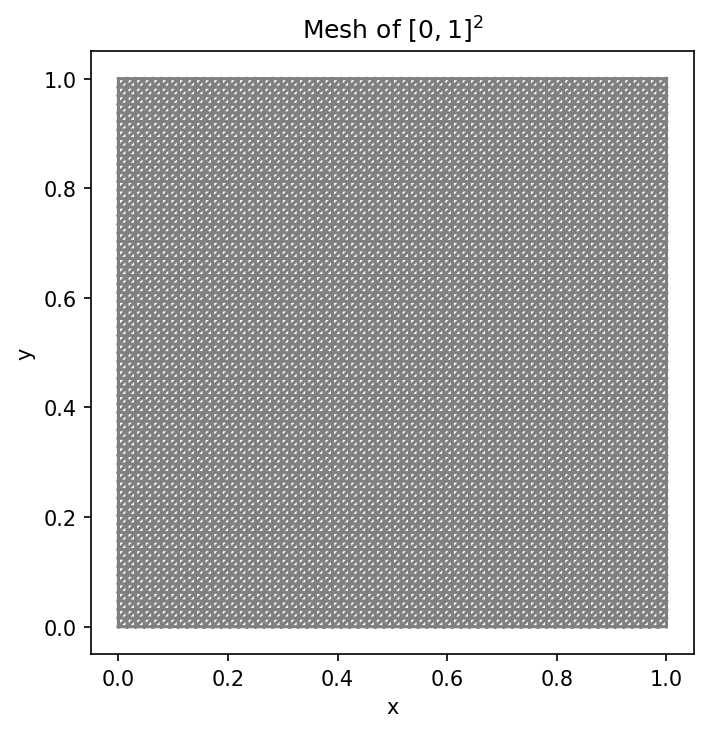
\includegraphics[width=0.4\textwidth]{mesh.png}\hfill
  
\includegraphics[width=0.4\textwidth]{omega.png}\\[4pt]
  
\includegraphics[width=0.4\textwidth]{y_d.png}\hfill
  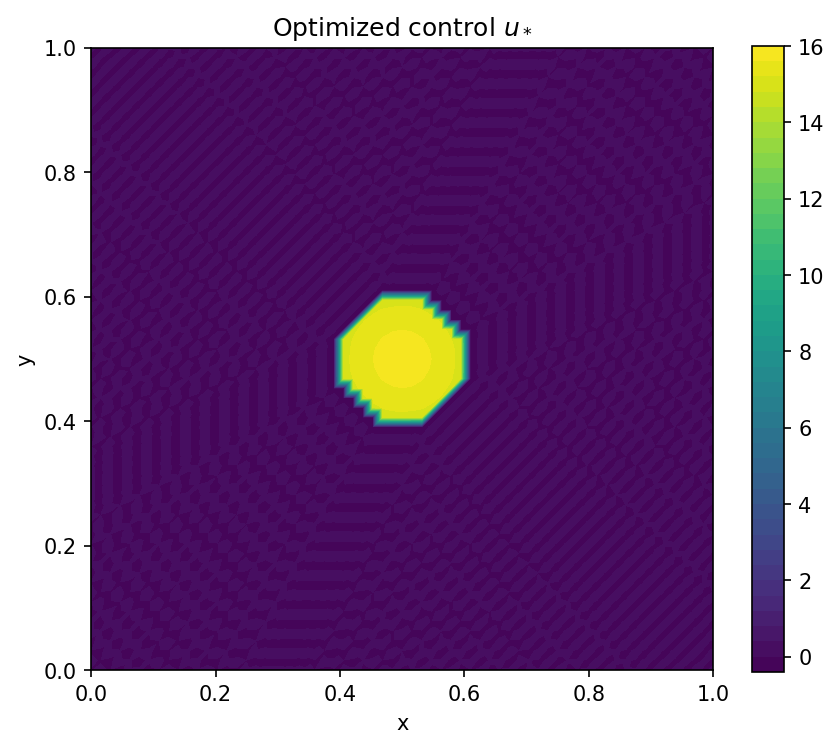
\includegraphics[width=0.4\textwidth]{u_opt.png}
  \caption{Top: mesh and control region $\omega$. Bottom-left: target $y_d$. Bottom-right: optimized control $u_*$.}
\end{figure}

\begin{figure}[h!]
  \centering
  
\includegraphics[width=0.45\textwidth]{y_opt.png}
  \caption{State $y(u_*)$ corresponding to the optimized control.}
\end{figure}

\begin{figure}[h!]
  \centering
  
\includegraphics[width=0.45\textwidth]{grad_norm.png}\hfill
  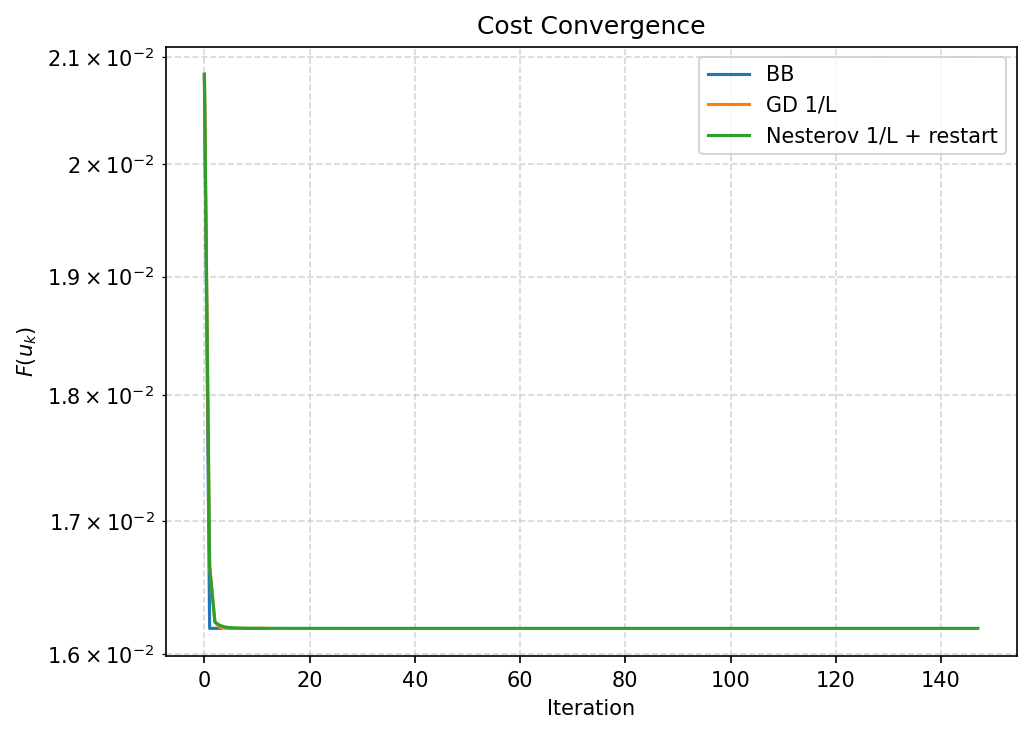
\includegraphics[width=0.45\textwidth]{cost.png}
  \caption{Convergence of gradient norm and objective for BB, GD with $1/L$, and Nesterov with restart.}
\end{figure}

\section{Conclusions}
The reduced formulation enables efficient first-order optimization by reusing sparse factorizations for state/adjoint solves. BB and Nesterov typically converge faster than fixed-step GD, while GD(1/L) provides a strong baseline when a reliable Lipschitz estimate is available.

\end{document}
